\chapter{Preliminaries}

%This chapter

%---------------------------------------------------------------------------------------------------------------------------------------------

\section{Negotiations}

Negotiations helps in modelling interactions from an observational point of view, where several partners come together to agree on one out of a number of possible outcomes (a synchronized nondeterministic choice). While such an interaction can be modelled in any standard model of concurrency, but the conventional automata-theoretic models focus on states and transitions, and specify how local states of agents determine global behaviours. In negotiations, the basic building blocks are the interactions between the agents, which are called atomic negotiations. After each atomic negotiation, the participating agents collectively agree on an outcome and move on to participate in other atomic negotiations. Atomic negotiations can be combined into distributed negotiations. For example, a distributed negotiation between a buyer, a seller, and a broker consists of one or more rounds of atomic negotiations involving the buyer and the broker, or the seller and the broker, followed by a concluding atomic negotiation between the buyer and the seller.

Apart from the modelling benefit, much can be gained by studying formal models of negotiations. The negotiation point of view reveals new classes of systems with polynomial analysis algorithms for problems like reachability, soundness etc. In this chapter we study the model of negotiations and discuss some interesting results about them.

The formal model for distributed negotiations is inspired by van der Aalst’s workflow Petri nets \cite{}. A negotiation atom, or just atom, involves a set of parties (for instance, buyer and broker), and has a set of possible outcomes (for example, buy and sell). Each party has a set of possible internal states, and each outcome has associated a state-transformer; if the parties agree on a given outcome, then its associated transformer determines the possible “exit states” of the parties after executing the atom as a function of their “entry states” before executing the atom. Atoms are combined into distributed negotiations, by means of a next-atoms function that determines for each atom, each party, and each outcome, the set of atoms the party is ready to engage in next if the atomic negotiation ends with that outcome. We assume that a distributed negotiation always starts with an initial atom, which involve all parties of the complete distributed negotiation.

%---------------------------------------------------------------------------------------------------------------------------------------------

\subsection{Syntax}

%Agents
We recall the definitions of \cite{} for syntax of \textit{negotiations}. Although we will not require the complete definition for the purpose of this thesis, we start with the complete syntax as given in \cite{}. We give an alternate definition in \ref{}, which we will use throughout the thesis.

Let $A$ be a finite set (of \textit{agents} or \textit{processes}), representing potential parties of a negotiation. Each agent $a \in A$ is a transition system with a (possibly infinite) nonempty set $Q_a$ of \textit{internal states} with a distinguished subset $Q_{0a} \subseteq Q_a$ of \textit{initial states}. We denote by $Q_A$ the cartesian product $\prod_{a \in A} Q_a$. So a state is represented by a tuple $(q_{a_1}, \dots, q_{a_{|A|}}) \in Q_A$. 

%---------------------------------------------------------------------------------------------------------------------------------------------

%Transformers
A \textit{transformer} is a left-total relation $\tau \subseteq Q_A \times Q_A$, representing a nondeterministic state transforming function. Given $S \subseteq A$, we say that a transformer $\tau$ is an $S$-transformer if, for each $a_i \notin S$, $((q_{a_1}, \dots, q_{a_{|A|}}),(q'_{a_1}, \dots, q'_{a_{|A|}})) \in \tau$ implies $q_{a_i} = q'_{a_i}$. So an $S$-transformer only transforms internal states of agents in $S$ or in a subset of $S$.

%---------------------------------------------------------------------------------------------------------------------------------------------

%Atomic negotiation
\begin{definition}[Atomic negotiation]
An \textsf{atomic negotiation}, or just an atom, over a set of agents $A$ is a triple $n = (P, R, \d)$, where $P \subseteq A$ is a nonempty set of parties or participants of $n, R$ is a finite, nonempty set (\textit{results}), and $\d$ is a mapping assigning to each result $r \in R$ a $P$-transformer $\d(r)$.
\end{definition}

$P_n, R_n$ and $\d_n$ will denote the components of an atom $n$. For each result $r \in R_n$, the pair $(n, r)$ is called an \textit{outcome}. The difference between results and outcomes is that the same result can belong to different atoms whereas the sets of outcomes are pairwise disjoint.

If the states of the agents before an atomic negotiation $n$ are given by a tuple $q$ and the result of the negotiation is $r$, then the agents change their states to $q'$ for some $(q, q') \in \d_n(r)$. Only the parties of $n$ can change their internal states. However, it is not required that a $P_n$-transformer $\d_n(r)$ actually changes the states of all agents in $P_n$. Each result $r \in R_n$ is possible, independent of the previous internal states of the parties of $n$.

%---------------------------------------------------------------------------------------------------------------------------------------------

%Start example
As a simple example, consider an atomic negotiation $n_{ab}$ with parties $a$ (ATM machine) and $b$ (bank). The goal of the negotiation is to determine whether an OTP received by the ATM machine from some customer is correct or not. The possible results are $\{match, fail\}$. The transformer $\d_{n_{ab}}$ includes: 

$$\d_{n_{ab}}(match) = \{(\texttt{match\_otp}, \texttt{waiting}) (\texttt{success}, \texttt{success})\}$$
$$\d_{n_{ab}}(fail) = \{(\texttt{match\_otp}, \texttt{waiting}) (\texttt{ask\_otp}, \texttt{waiting})\}$$

%%%%%%%%%%%%%%%%%%%%%%%%%%%%%%%%%%%%%%%%%%%%%%%%%%%%%%

%---------------------------------------------------------------------------------------------------------------------------------------------

%Combining atomic negotiation
\begin{definition}
Given a finite set of agents $A$ and a finite set of atoms $N$ over $A$, let $T(N)$ denote the set of triples $(n, a, r)$ such that $n \in N$, $a \in P_n$, and $r \in R_n$. A (distributed) negotiation is a tuple $N = (N, n_0, n_f, \chi)$, where $n_0, n_f \in N$ are the initial and final atoms, and $\chi : T(N) \xra{} 2^N$ is the transition function. Further, $N$ satisfies the following properties:
\begin{enumerate}
	\item every agent of $A$ participates in both $n_0$ and $n_f$;
	\item for every $(n, a, r) \in T(N): \chi(n, a, r) = \emptyset$ iff $n = n_f$.
\end{enumerate}
The graph associated with $N$ has vertices $N$ and edges $\{(n, n') \in N \times N \mid \exists (n, a, r) \in T(N) : n' \in \chi(n, a, r)\}$.
\end{definition}

The initial and final atoms mark the beginning and the end of the negotiation (and sometimes this is their only role). We may have $n_0 = n_f$. In this case, due to $(2)$, $N = \{n0\}$, i.e, the negotiation has only one single atom. Notice that $n_f$ has, as all other atoms, at least one result $\textsf{end} \in R_{n_f}$.

%---------------------------------------------------------------------------------------------------------------------------------------------

%Continue example

%---------------------------------------------------------------------------------------------------------------------------------------------

\subsection{Negotiations: alternate definition}

%Our purpose
Internal states of agents and their transformers won’t play an important role in this thesis. Internal states do not influence behaviour in negotiations, i.e., we can consider the control flow and data aspects separately. In this thesis we only need the control flow aspect. Hence, we give a simpler definition below, which suits our purpose.

%---------------------------------------------------------------------------------------------------------------------------------------------

%Definition for our purpose
\begin{definition}
Let $P$ be a finite set of agents, $\S$ a finite set of outcomes. A \textsf{negotiation} $\mathcal{N}$ is given by a tuple $(N, dom, \delta)$ where
\begin{itemize}
\item $N$ is a finite set of nodes (also called atomic negotiations),
\item $dom : N \rightarrow \mathcal{P}(P)$ maps each node to a non-empty subset of agents; we assume $dom(n_{in})=P$, where $n_{in}$ is the initial node,
\item $\delta = {\delta_p}_{p \in P}$ is a tuple of transition relations, one for each agent, where $\delta_p : N_p \times \S \rightarrow \mathcal{P}(N_p)$ maps each node-outcome pair (n, a) to a set of nodes $M \subseteq N_p$ that $p$ becomes ready to engage in after this outcome; we will call node-outcome pairs $(n, a)$ as \textit{locations}.
\end{itemize}
\end{definition}

%---------------------------------------------------------------------------------------------------------------------------------------------

%Semantics
\subsection{Semantics}

A \textsf{marking} of a negotiation $\mathcal{N} = (N,dom,\delta)$ is a mapping $x: A \rightarrow \mathcal{N}$. Intuitively, $\delta(p)$ is the set of nodes that agent $p$ is currently ready to engage in next. The initial and final markings, denoted by $x_0$ and $x_f$ respectively, are given by $x_0(p) = {n0}$ and $x_f(p) = \emptyset$ for every $p \in A$. 

A marking \textsf{enables} an atom $n$ if $n \in x(p)$ for every $p \in P_n$, i.e., if every party of $n$ is currently ready to engage in it. If $x$ enables $n$, then $n$ can take place and its parties agree on a result $r$; we say that the outcome $(n, r)$ \textsf{occurs}. The occurrence of $(n, r)$ produces a next marking $x'$ given by $x'(p) = \delta(n,p,r)$ for every $p \in P_n$, and $x'(p) = x(p)$ for every $p \in A \setminus P_n$. We write $x \xrightarrow{(n,r)} x'$ to denote this, and call it a \textsf{small step}.

We write $x \xrightarrow{\sigma}$ to denote that there is a sequence $x_0 \xrightarrow{(n_0,r_0)} x_1 \xrightarrow{(n_1,r_1)} \cdots \xrightarrow{(n_k,r_k)} x_{k+1} \cdots$ of small steps such that $\sigma = (n_0, r_0) (n_1, r_1)\dots(n_k, r_k)\dots$. We call $\sigma$ an \textsf{occurrence sequence} from marking $x_0$. If $\sigma$ is finite and ends with $(n_k,r_k)$, then we write $x_k \xrightarrow{\sigma} x_{k+1}$ and say that $x_{k+1}$ is reachable from $x_0$. If $x_0$ is the initial marking, then we call $\sigma$ an initial occurrence sequence. If moreover $x_{k+1}$ is the final marking, then $\sigma$ is a \textsf{large step}.

Given an agent $p$, we always have that either $x(p) = \{n_0\}$ or $x(p) = \delta(n,p,r)$ for some atom $n$ and result $r$. The marking $x_f$ can only be reached by the occurrence of an outcome $(n_f,r)$, where $n_f$ is the final atom and thus $r$ is a final result. It does not enable any atom. Any other marking that does not enable any atom is a \textsf{deadlock}. A marking which is reachable from itself but from which the final marking is not reachable is a \textsf{livelock}.

Reachable markings are graphically represented by placing tokens (black dots) on the forking points of the hyperarcs (or, if the hyperarc consists of just one arc, in the middle of the arc).

The behaviour of a negotiation is described by its reachability graph.

\begin{definition}
The \textsf{reachability graph} or \textsf{marking graph} of a negotiation $\mathcal{N}$ has all markings reachable from $x_0$ as vertices, and an arc leading from $x$ to $x'$ and annotated by $(n, r)$ whenever $x \xrightarrow{(n,r)} x'$. The initial marking $x_0$ is the distinguished initial vertex.
\end{definition}

\subsubsection{Graphical representation}
Negotiations admit a graphical representation. A node (atomic negotiation) $n$ is represented as a black bar with a white circles, called ports, one for each process in $\dom(n)$. So, for example, the negotiation of Figure~\ref{} has seven nodes $n_{in}, n_0, \dots, n_6$. Nodes $n_{in}, n_3$, and $n_6$ have three ports each, while nodes $n_1, n_2, n_4$ and $n_5$ have two ports. A transition $\delta_p(n,a) = {n_1,\dots,n_k}$ is represented by a hyper-arc, labeled by $a$, that connects the port of process $p$ in $n$ with the ports of process $p$ in $n_1,\dots,n_k$. In particular, for the negotiation Figure~\ref{} we have $\calA = \{c, a, b\}, N = n_{in}, n_0, \dots, n_6, \S = \{st, req, det, e\_otp, match, fail, g\_up\}$, and, for example $\dom(n_1) = \{c, a\}, \dom(n_3) = \{c, a, b\}, \delta_c(n_1,req) = \{n_3\}$ and $\delta_b(n_5, fail) = \{n_5\}$. $\delta_c(n_4, e\_otp) = \{n_4, n_6\}$ is a proper hyper-arc in Figure~\ref{}.

\subsubsection{A motivating example}

We use the example in Figure~\ref{fig:ATM} to introduce our model informally.  Consider a time-constrained transaction in an ATM machine ($a$), where a customer ($c$) wants to reset her ATM PIN via an OTP received from her bank ($b$).  Here, $a$, $c$, and $b$ are the \emph{agents} in the system. Their direct interactions are represented by thick horizontal lines, called nodes. After each interaction, the participating agents decide on an outcome, represented by arrows. Initially, all agents are in the node $n_{in}$ node. They choose the outcome $st$ to start the transaction. Agents $a$ and $c$ go to node $n_1$ and $b$ goes to $n_2$.The customer gives her card details and requests for a PIN change in the ATM at  node $n_1$ by choosing the outcome $req$. At $n_2$, the ATM conveys this request to the bank and sends the details through the outcome $det$. The bank and the customer talk to each other at $n_3$, and $b$ sends an OTP to the customer through the outcome $s\_otp$. At $n_4$, the customer enters the OTP in the ATM. After entering the OTP, shown by the outcome $e\_otp$ the customer is ready to engage with the ATM either at $n_4$ or at $n_6$, represented by the non-deterministic arc leading to $n_4$ and $n_6$. The ATM talks to the bank at $n_5$ to check the OTP. If it matches, the ATM goes to $n_6$, otherwise it goes back to $n_4$.

\begin{figure}[t]
\centering
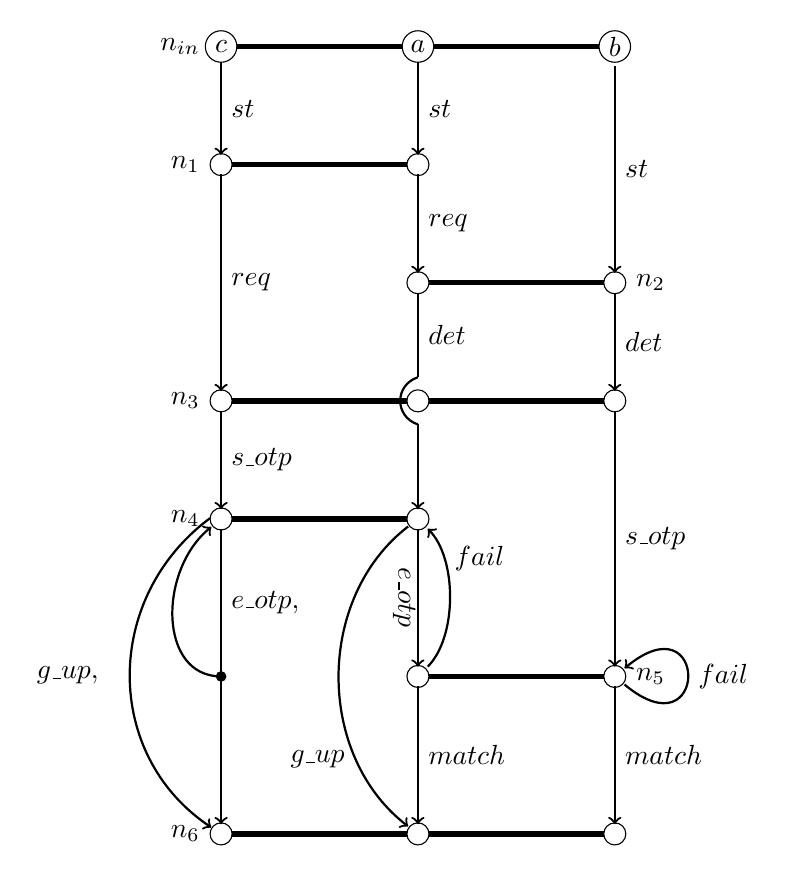
\begin{tikzpicture}

\begin{scope}[line width=2pt]
\draw (0.,0) node [left] {$n_{in}\,\,$} -- (5,0);
\draw (0.,-1.5) node [left] {$n_{1}\,\,$} -- (2.5,-1.5);
\draw (2.5,-3) -- (5,-3) node [right] {$\,\,n_{2}$};
\draw (0.,-4.5) node [left] {$n_{3}\,\,$} -- (5,-4.5);
\draw (0.,-6) node [left] {$n_{4}\,\,$} -- (2.5,-6);
\draw (2.5,-8) -- (5,-8)  node [right] {\,\,$n_{5}$};
\draw (0.,-10) node [left] {$n_{6}\,\,$} -- (5,-10);
\end{scope}

\begin{scope}[fill=white]
\filldraw  (0,0)  circle (2mm) node (nic) {$c$};
\filldraw  (2.5,0)  circle (2mm) node (nia) {$a$};
\filldraw  (5,0)  circle (2mm) node (nib) {$b$};

\filldraw  (0,-1.5)  circle (1.4mm) node (n1c) {};
\filldraw  (2.5,-1.5)  circle (1.4mm) node (n1a) {};

\filldraw  (2.5,-3)  circle (1.4mm) node (n2a) {};
\filldraw  (5,-3)  circle (1.4mm) node (n2b) {};

\filldraw  (0,-4.5)  circle (1.4mm) node (n3c) {};
\filldraw  (2.5,-4.5)  circle (1.4mm) node (n3a) {};
\filldraw  (5,-4.5)  circle (1.4mm) node (n3b) {};

\filldraw  (0,-6)  circle (1.4mm) node (n4c) {};
\filldraw  (2.5,-6)  circle (1.4mm) node (n4a) {};

\filldraw  (2.5,-8)  circle (1.4mm) node (n5a) {};
\filldraw  (5,-8)  circle (1.4mm) node (n5b) {};

\filldraw  (0,-10)  circle (1.4mm) node (n6c) {};
\filldraw  (2.5,-10)  circle (1.4mm) node (n6a) {};
\filldraw  (5,-10)  circle (1.4mm) node (n6b) {};

\filldraw  [fill=black] (0,-8)  circle (0.6mm) node (v1) {};

\end{scope}

\begin{scope}[thick,->]

\draw (nic) -- (n1c) node [right, midway] {$st$};
\draw (n1c) -- (n3c) node [right, midway] {$req$};
\draw (n3c) -- (n4c) node [right, midway] {$s\_otp$};
\draw (n4c) -- (n6c) node [right, text width = 1.5 cm, near start] {$e\_otp,$};
\draw (0,-8) .. controls  (-0.8,-8) and (-0.8,-6.65) .. (n4c) node [left, midway] {};

\draw (nia) -- (n1a) node [right, midway] {$st$};
\draw (n1a) -- (n2a) node [right, midway] {$req$};
\draw (2.5,-4.8) -- (n4a);
\draw (n4a) -- (n5a) node [below=-0.1cm, sloped, midway] {$e\_otp$};
\draw (n5a) -- (n6a) node [right, text width = 1 cm, midway] {$match$};
\draw (n5a) .. controls (3,-7.5) and (3,-6.5) .. (n4a) node [right, near end] {$fail$};
\draw (n4a) .. controls  (1.2,-7) and (1.2,-9) .. (n6a) node [left=-0.3cm, text width = 1 cm, near end] {$g\_up$};

\draw (nib) -- (n2b) node [right, midway] {$st$};
\draw (n2b) -- (n3b) node [right, midway] {$det$};
\draw (n3b) -- (n5b) node [right, text width = 1 cm, midway] {$s\_otp$};
\draw (n5b) -- (n6b) node [right, text width = 1 cm, midway] {$match$};
\draw (n5b) .. controls  (6.2,-9) and (6.2,-7) .. (n5b) node [right, midway] {$fail$};

\draw (n4c) + (-0.14,0.01) .. controls  (-1.5,-7) and (-1.5,-9) .. (n6c) node [left=-0.2cm, text width = 1.25 cm, midway] {$g\_up,$};

\end{scope}

\draw [thick] (n2a) -- (2.5,-4.2) node [right, midway] {$det$};
\draw [thick] (2.5,-4.2) .. controls (2.2,-4.3) and (2.2,-4.7) .. (2.5,-4.8);
\end{tikzpicture}
\caption{A local-timed negotiation modeling a transaction between a customer, an ATM and a bank}
\label{fig:ATM}
\end{figure}

%---------------------------------------------------------------------------------------------------------------------------------------------

%Reachability graphs
An occurrence sequence of a negotiation can be arbitrarily long. Therefore, the set of possible occurrence sequences can be infinite. Since we have markings and steps, an obvious way to describe behaviour with finite means is by reachability graphs:

\begin{definition}
The reachability graph of a negotiation $\Nn$ has all markings reachable from $x_0$ as vertices, and an arc leading from $x$ to $x'$ and annotated by $(n, r)$ whenever $x \xra{(n, r)} x'$. The initial marking $x_0$ is the distinguished initial vertex.
\end{definition}

Generally, atoms with disjoint sets of parties can proceed concurrently, whereas atoms sharing a party cannot. Formally, if two outcomes $(n_1, r_1)$ and $(n_2, r_2)$ are enabled by the same reachable marking $x$ and $P_{n_1} \cap P_{n_2} = \emptyset$ then the outcomes can occur concurrently. The condition $P_{n_1} \cap P_{n_2} = \emptyset$ is also necessary for concurrent occurrences of outcomes because, in our model, a single agent cannot be engaged concurrently in two different atoms, and because two state transformers cannot operate concurrently on the local state of an agent. Thus concurrency between outcomes depends only on the involved atoms (and their parties) and not on the results. 

Concurrency is formally captured by the \textit{concurrent step reachability graph}, defined next. A \textit{concurrent step} enabled at a reachable marking $x$ is a nonempty set of pairwise concurrent outcomes, each of them enabled by $x$. It is immediate to see that all the outcomes of a concurrent step can be executed subsequently in arbitrary order and that the marking finally reached does not depend on the chosen order. We call this marking \textit{reached by the concurrent step}.

\begin{definition}
The \textsf{concurrent step reachability graph} of a negotiation $\Nn$ has all markings reachable from $x_0$ as vertices. An arc, annotated by a nonempty set of outcomes, leads from $x$ to $x'$ whenever the outcomes of this set are pair-wise concurrent and the concurrent step leads from $x$ to $x'$. Again, $x_0$ is the distinguished initial vertex.
\end{definition}

%\subsubsection{Semantics as trace}

%We can view a run of negotiation as a \emph{trace} over the events of the run. Figure~\ref{} gives an example of a trace for the negotiation depicted in Figure~\ref{} and described in Example~\ref{}. Fix a negotiation $\Nn$.
%Suppose we are given a run $\rho:= C_1 \xra{e_1} C_2 \xra{e_2} \cdots C_k$, starting from some arbitrary configuration $C_1$. 

%\paragraph*{From run to trace.} The trace $\tr(\rho)$ is a directed graph $(E_\rho, \{\xra{}_p\}_{p\in \calA})$ equipped with an assignment $\{\tau^0_p\}_{p\in \calA}$ gives an initial local-time for each agent:
%\begin{itemize}
%\item the vertex set $E_\rho$ is given by the set of events $\{e_1, e_2, \dots, e_{k-1}\}$ along with special events $\{\bot_p\}_{p\in \calA}$ denoting an initial event for each agent; in Figure~\ref{fig:trace}, the initial events $\bot_p$ are denoted by dots. 
%\item the edge relation is partitioned as $\{\xra{}_p\}_{p \in \calA}$; there is an edge $e_i \xra{~\theta~}_p e_j$ with label $\theta$ if $e_j$ is the next event that $p$ participates after $e_i$, and $\theta$ is the time spent by $p$ in between. Formally, we have $i < j$, $p \in \dom(e_i) \cap \dom(e_j)$, and there is no $i < i'< j$ such that $p \in \dom(e_{i'})$; moreover, $\theta = \Delta_{j-1}(p)$, which is indeed the time spent by agent $p$ between the events $e_i$ and $e_j$ --- this is because of our hypothesis on the run $\rho$ that local delay $\Delta_{\ell}(p)$ is non-zero only if $p$ participates in $e_\ell$ (cf. Remark~\ref{rem:runs}). 
%\end{itemize}
%Given a trace with its initial assignment of local-times, we can compute a local-time for each agent at each event $e$, by summing up the initial local time and the delays along the $\xra{}_p$ edges starting from $\bot_p$ to $e$. For an event $e$ and an agent $p \in \dom(e)$, we will write $\tau_p(e)$ for this timestamp. For example, in Figure~\ref{fig:trace}, all initial timestamps are $0$, and we have $\tau_p(a) = 1$, $\tau_p(b) = \tau_q(b) = 2$. 

%\paragraph*{From trace to run.} We have seen how to get a trace $\tr(\rho)$ from a run $\rho$. For the reverse, given a trace $\tr$ and an initial configuration $(C_0, v_0)$ that matches with the initial timestamps $\tau^0_p$ of $\tr$, i.e. $v_0(t_p) = \tau^0_p$ for all agents $p$, we can derive run $\rho[(C_0, v_0), \tr]$ as follows: to each event $e$ a step $\Delta_e$ can be associated, where for each $p \in \dom(e)$, $\Delta_e(p)$ is the label of the incoming $\xra{}_p$ edge to $e$, and for $p \notin \dom(e)$, we set $\Delta_e(p)$ to $0$; then we get a run by starting with $(C_0, v_0)$, linearizing the events of $\tr$, executing the corresponding steps, and computing intermediate configurations of the LTN. The sequence $\rho[(C_0,v_0), \tr]$ gives a run of the LTN if all the events of the trace can be executed this way.

\subsection{Examples}

Here we give some more examples.

% a^nb^nc^n

% all k-bit binary numbers

%------------------------------------------------------------------------------------------------------------------------------------------

\subsection{Reachability problem and complexity results}

%------------------------------------------------------------------------------------------------------------------------------------------

\subsection{Relation with PN}

%------------------------------------------------------------------------------------------------------------------------------------------

\section{Time and concurrency}

\subsection{Timed automata}

We assume the framework of dense time and consider as time domain the set $\Rpos$ of non-negative reals. Let $\S$ be a finite alphabet. A timed word over $\S$ is a finite or infinite sequence of pairs $(a_0,t_0)(a_1,t_1)\cdots$ such that for every $i \in N$, $a_i \in \S$, and $(t_i)$ is a non-decreasing sequence in $\Rpos$. Furthermore we may call $t_i$ the timestamp of $a_i$. 

Let $X$ be a finite set of variables, called clocks. A (clock) valuation over $X$ is a mapping $v : X \rightarrow \Rpos$ that assigns to each clock a time value. Let $d \in \Rpos$, the valuation $v + d$ is defined by $(v + d)(x) = v(x) + d$ for every $x \in X$. For $Y \subseteq X$, we denote by $[Y]v$ the valuation assigning $0$ for all $x \in Y$, where the set of clocks $Y$ are \textit{reset}, and sets $x$ to $v(x)$ otherwise. For a valuation $v$ and a clock $x$, we denote the integral part of $v(x)$ by $\lceil v(x) \rceil$ and the fractional part of $v(x)$ by $\{v(x)\}$.

The set of clock constraints over $X$, denoted $C(X)$, is defined by the grammar: $g:= x \bowtie c \mid g \wedge g$, where $x \in X$, $\bowtie \in \{<, \leq, =, \geq, >\}$, and $c \in \N$.

\begin{definition}[Timed automaton \cite{}]
A \textsf{Timed Automaton (TA)} is a tuple $A = (Q, \S, X, T, q_0, Acc)$ where
\begin{itemize}
	\item $Q$ is a finite set of states,
	\item $\S$ is a finite alphabet,
	\item $X$ is a finite set of clocks,
	\item $q_0 \in Q$ is the initial state,
	\item $Acc \subseteq Q$ is a set of accepting states,
	\item $T \subseteq Q \times \S \times C(X) \times 2^X \times Q$ is a finite set of transitions $(q, a, g, R, q')$ where $a$ is a letter in $\S$, $g$ is a clock constraint called the \textit{guard}, and $R$ is the set of clocks that are reset on the transition.
\end{itemize}
\end{definition}

The behaviour of a timed automaton is described by a graph as in Figure~\ref{}. We will call it the semantics of a timed automaton. Here is the formal definition of this infinite graph.

\paragraph*{Semantics of a timed automata.} Let $\calA$ be a timed automaton. The semantics of $\calA$ is given by a transition system $S_\calA$ whose nodes are configurations $(q, v)$ consisting of a state $q$ of $\calA$ and a valuation $v$ giving the values of clocks. The initial configuration is given by $(q_0, \textbf{0})$ with $q_0$ being the initial state of $\calA$, and $\textbf{0}$ is the zero vector. The transition relation $\xra{}$ is a union of two kinds of transitions:

\textbf{delay} $(q, v) \xra{\delta} (q, v + \delta)$ for some $\delta \in \Rpos$;

\textbf{action} $(q, v) \xra{t} (q', v')$ for some transition $t = (q, a, g, R, q') \in T$ such that $v \models g$ and
$v' = [R]v$.

A \textsf{run} of $\calA$ is a finite sequence of transitions starting from the initial configuration $(q_0, \textbf{0})$. Without loss of generality, we can assume that the first transition is a delay transition and that delay and action transitions alternate. We write $(q, v) \xra{\d, t} (q', v')$ if there is a delay transition $(q, v) \xra{\d} (q, v + \d)$ followed by an action transition $(q, v + \d) \xra{t} (q', v')$. So a run of $\calA$ can be written as: $(q_0, v_0) \xra{\d_0, t_0} (q_1, v_1) \xra{\d_1, t_1} \cdots \xra{\d_{n-1}, t_{n-1}} (q_n, v_n)$, where $(q_0, v_0)$ represents the initial configuration $(q_0, \textbf{0})$. A run is accepting if it ends in a configuration $(q_n, v_n)$ with $q_n \in Acc$.

\subsubsection{Regions}

Since the transition system determined by an automaton is infinite, the standard solution is to find a finite approximation of this transition system by grouping valuations together. The grouping should be done in such a way that $v$ and $v'$ are in the same group if all the states of the automaton that are reachable from $(q, v)$ and $(q, v')$ are the same, for all $q$. That is, if there is the following run from $(q, v)$: $(q_0, v_0) \xra{\d_0, t_0} (q_1, v_1) \xra{\d_1, t_1} \cdots \xra{\d_{n-1}, t_{n-1}} (q_n, v_n)$, then there should be a run with the same sequence of discrete states $q_1, \dots ,q_n$ from $(q, v')$. That is, there exist $\d_0, \dots, \d_{n-1} \in \Rpos$ such that the following is a valid run from $(q, v')$: $(q_0, v_0) \xra{\d_0, t_0} (q_1, v_1) \xra{\d_1, t_1} \cdots \xra{\d_{n-1}, t_{n-1}} (q_n, v_n)$.

Note that for the emptiness problem, we do not care about the intermediate times spent in a run. We just insist that $v'$ should be able to take the same sequence of transitions as $v$. One such grouping is given by the region abstraction \cite{}. The space of valuations is partitioned into a finite number of regions. Two valuations within a region are indistinguishable with respect to reachability. Having formed these finite number of regions, a cross product with the states of the automaton is taken to give state-augmented regions. These state-augmented regions act as nodes of what is called the region graph of the automaton whose transitions are defined in a natural way, using the valuations present in the region. The analysis of the automaton is then performed using this finite region graph. 

Let $X$ be a finite set of clocks. Let $M : X \xra N \cup \{-\infty\}$ be a bound function that associates a constant $M_x \in N$ to every clock $x$.

\begin{definition}[Region equivalence \cite{}]
Two valuations $v, v' \in \Rpos$ are region equivalent w.r.t. $M$, denoted $v \sim_M v'$ iff for every $x, y \in X$:
\begin{itemize}
	\item $v(x) > M_x$ iff $v'(x) > M_x$;
	\item if $v(x) \leq M_x$, then $\lceil v(x) \rceil = \lceil v'(x) \rceil$;
	\item if $v(x) \leq M_x$, then $\{v(x)\} = 0$ iff $\{v'(x)\} = 0$;
	\item if $v(x) \leq M_x$ and $v(y) \leq M_y$ then $\{v(x)\} \leq \{v(y)\}$ iff $\{v'(x)\} \leq \{v'(y)\}$.
\end{itemize}
\end{definition}

Given a timed automaton $A$, a bound function is obtained by choosing for a clock $x$, the maximum constant appearing in a guard involving $x$. Then, the first three conditions in the above definition ensure that the two valuations satisfy the same guards. The last one enforces that for every $\d \in \Rpos$ there is $\d' \in \Rpos$, such that valuations $v + \d$ and $v' + \d'$ satisfy the same guards.

\begin{definition}[Regions \cite{}]
Let $M : X \xra{} \N \cup \{-\infty\}$ be a bound function. A region is an equivalence class of $\sim_M$. We write $[v]^M$ for the region of $v$, and $\calR_M$ for the set of all regions with respect to $M$.
\end{definition}

Figure~\ref{} shows the division into regions when there are two clocks $x$ and $y$. We also give below a constructive definition of regions which would be useful to estimate the number of regions.

\begin{definition}[Region: constructive definition \cite{}]
A region with respect to bound function $M$ is a set of valuations specified as follows:
\begin{itemize}
	\item for each clock $x \in X$, one constraint from the set: $\{x = c \mid c = 0, \dots, M_x\} \cup \{c - 1 < x < c \mid c = 1, \dots, M_x\} \cup \{x > M_x\}$
	\item for each pair of clocks $x, y$ having interval constraints: $c - 1 < x < c$ and $d - 1 < y < d$, it is specified if $\{x\}$ is less than, equal to or greater than $\{y\}$.
\end{itemize}
\end{definition}

If $r$ is a region then we will write $r \models g$ to mean that every valuation in $r$ satisfies the guard $g$. It is straightforward to see that if a valuation $v \in r$ satisfies the guard $g$, then every valuation $v' \in r$ satisfies $g$. We will now show the other property with respect to time-elapse mentioned above.

\begin{lemma}
Let $v, v'$ be valuations such that $v' \sim v$. Then, for all $\d' \in \Rpos$ there exists a $\d' \in \Rpos$ such that $v' + \d' \sim_M v + \d$.
\end{lemma}

\begin{proof}
We know $v' \sim v$ and we are given $\d$. We need to choose $\d'$. Put $\lceil \d' \rceil$ to be $\lceil \d \rceil$. Clearly, we have $v' + \lceil \d' \rceil \sim_M \lceil \d \rceil$: that is, valuations $v' + \lceil \d' \rceil$ and $v + \lceil \d \rceil$ have the same integral parts and the same ordering of fractional parts (modulo $M$). Let $x_1 \lessdot_1 x_2 \lessdot_2 \cdots \lessdot_{k - 1} x_k$ be the ordering of fractional parts of clocks less than $M$ in both the valuations. Here $\lessdot$ denotes either $<$ or $=$. 

From $v + \lceil \d \rceil$, elapsing a fractional amount $\{\d\}$ might move some of the clocks up to the next integer. Let $x_j, x_{j + 1}, \dots, x_k$ be the clocks that have their integral values increased from $v + \lceil \d \rceil$ due to the fractional elapse $\{\d\}$. Thanks to the denseness of the real line, one can choose $\{\d'\}$ between the fractional values of clocks $x_{j - 1}$ and $x_j$ in $v' + \lceil \d' \rceil$ so that $v' + \d'$ has the same integers as $v + \d$ and the same ordering of fractional parts (modulo $M$).
\end{proof}

Given a bound function $M$, the number of regions in $\calR_M$ is finite. Once this finite partition of the valuations is obtained, we proceed to define a finite graph built from these regions, that captures the behaviour of the timed automaton. For an automaton $A$, to define its region graph, we consider a bound function $M_A$ that is obtained from the automaton’s definition.

\begin{definition}[Maximal bounds]
Given an automaton $A$, the maximal bounds function $M_A: X \xra{} \N \cup \{-\infty\}$ associates to each clock $x$ the biggest constant appearing in a guard of the automaton that involves $x$. If there is no guard involving $x$, then $M_A(x)$ is assigned $-\infty$.
\end{definition}

We define the region graph of an automaton $A$ using the $\sim_{M_A}$ relation. Note that in class, we used the terminology region automaton. As we are not interested in the language accepted by this automaton, and instead we care if there is a path to the accepting state, we will stick to calling this a region graph.

\begin{definition}[Region graph \cite{}]
Nodes of the region graph denoted by $RG(A)$ are of the form $(q, r)$ for $q$ a state of $A$ and $r \in \calR_{M_A}$ a region. There is a transition $(q, r) \xra{t} (q', r')$ if there are $v \in r, \d \in \Rpos$ and $v' \in r'$ with $(q, v) \xra{\d, t} (q', v')$. The initial node of the region graph is $(q_0, [0]_{\sim_{M_A}})$ where $[0]_{\sim_{M_A}}$ represents the region to which the initial valuation $0$ belongs to. A node $(q, r)$ is said to be an accepting node if $q \in Acc$.
\end{definition}

Observe that a transition in the region graph is not decorated with a delay. Figure~\ref{} shows a part of the region graph $RG(A_1)$ of the automaton $A_1$ shown in Figure~\ref{}. It will be important to understand the property of pre-stability of regions \cite{}.

\begin{lemma}[Pre-stability of regions]
Let $A$ be an automaton. Transitions in $RG(A)$ are pre-stable: in each transition $(q,cr) \xra{t} (q', r')$, for every $v \in r$ there is a $\d \in \Rpos$ and a valuation $v' \in r'$ such that $(q, v) \xra{\d, t} (q', v')$.
\end{lemma}

\begin{proof}
By definition of the region graph, a transition $(q_1, r_1) \xra{t} (q_2, r_2)$ exists in $RG(A)$ if there are $v_1 \in r_1$, $\d \in \Rpos$ and $v_2 \in r_2$ with $(q_1, v_1) \xra{\d, t} (q_2, v_2)$. Let the transition $t$ be $(q_1, g, R, q_2)$. Pick a valuation $v'_1 \in r_1$. By Lemma~\ref{}, there exists a $\d'$ such that $v_1 + \d$ and $v'_1 + \d'$ belong to the same region. We know that valuations within the same region satisfy the same guards. Therefore since $v_1 + \d \models g$, we get that $v'_1 + \d' \models g$ too. From the definition of region equivalence, we get that regions are stable under projection to a subset of clocks and in particular, this entails that $[R](v'_1 + \d')$ belongs to the same region as $[R](v_1 + \d)$. We will now establish the correspondence between paths of the region graph and runs of the automaton. Consider two sequences 
$$(q_0, v_0) \xra{\d_0, t_0} (q_1, v_1) \xra{\d_1, t_1} \cdots (q_n, v_n)$$
$$(q_0, r_0) \xra{t_0} (q_1, r_1) \xra{t_1} \cdots (q_n, r_n)$$
where the first is a run in $A$, and the second is a path in $RG(A)$. We say that the first is an instantiation of the second if $v_i \in r_i$ for all $i \in \{1, \dots, n\}$. Equivalently, we say that the second is an abstraction of the first. The following lemma is a direct consequence of the pre-stability property.
\end{proof}

\begin{lemma}
Every path in $RG(A)$ is an abstraction of a run of $A$, and conversely, every run of $A$ is an instantiation of a path in $RG(A)$.
\end{lemma}

The above lemma shows that the region graph is sound and complete for state reachability.

\begin{theorem}[\cite{}]
Automaton $A$ has an accepting run iff there is a path in the region graph $RG(A)$ starting from its initial node to an accepting node.
\end{theorem}

While this theorem gives an algorithm for solving our problem, it turns out that this method is very impractical. The number of regions obtained using a bound function $M$ is $\calO (|X|! \cdot 2^{|X|} \cdot \prod_{x \in X} (2M_x + 2))$ \cite{} and constructing all of them, or even searching through them on-the-fly, has proved to be very costly.

\subsection{Network of timed automata}

\begin{definition}[Network of timed automata]\label{df:network}
    A network of timed automata with $k$ processes, is a $k$-tuple of
    timed automata $A_1,\dots,A_k$.  Each process
    $A_p=\struct{Q_p,\S_p,X_p,q^\init_p,T_p}$ has a finite set of states
    $Q_p$, a finite alphabet of actions $\S_p$, a finite set of clocks
    $X_p$, an initial state $q^\init_p$, and transitions
    $T_p\incl\S_p\times Q_p\times \phi(X_p)\times 2^{X_p}\times Q_p$.  We
    require that the sets of states, and the sets of clocks are pairwise
    disjoint: $Q_{p_1}\cap Q_{p_2}=\es$, and $X_{p_1}\cap X_{p_2}=\es$
    for $p_1\not=p_2$. We write $\Proc$ for the set of all processes.
  \end{definition}
  
  \begin{remark}
    In our definition each component has only one transition for each action. This allows some notational convenience. Since we will be interested in the reachability property, this is not a restriction, as we can always introduce new actions.
  \end{remark}

  We will use the following abbreviations: $Q=\Pi_{p=1}^k Q_p$, $\Ss=\bigcup_{p=1}^k \Ss_p$ and $X=\bigcup_{p=1}^k X_p$.
    
  We define the domain of an action $a \in \Sigma$, denoted as $\dom(a)$, as
  the set of timed processes participating
  in the action $a$.
  Formally, $\dom(a) = \{i \mid a \in \Sigma_i\}$.
  A transition whose domain contains more than one element is called a
  \emph{synchronization transition}.
  A synchronization action could have guards and resets in each participating component.
  If the guard of a synchronization transition in a component of the network
  is satisfied, we say that the transition is \emph{locally enabled} in that
  component.
  
  
  Next, we define the semantics of a network of timed automata. 
  \begin{definition}[Global-time semantics]\label{def:global-run}
      The semantics of a network $\Aa$ is given by a transition system $\Gg_{\Aa}$
      whose states are configurations $(q, v)$. 
      The set of initial states is given by configurations $(q^\init, v^\init)$ where $q^\init(p)=q_p^\init$ is the tuple of initial states, and $v^\init = v_0$ is an initial valuation.
    
      There are two kinds of
      transitions, which we call steps: global delay, and action steps.  A
      \emph{global delay} by the amount $\d\in\Rpos$ gives a step
      $(q,v)\step{\d}(q,v+\d)$.  An \emph{action step} on action $b$ gives
      $(q,v)\step{b}(q',v')$ if there is a set of $b$-transitions
      $\set{(q_p,g_p,R_p,q'_p)}_{p\in\dom(b)}$ of the respective processes
       such that:
      \begin{itemize}
        \item  processes from $\dom(b)$ change states: $q_p=q(p)$, $q'_p=q'(p)$, for
        $p\in\dom(b)$, and $q(p)=q'(p)$  for $p\not\in\dom(b)$; 
        \item all the guards are satisfied: $v\sat g_p$, for $p\in\dom(b)$;
        \item all resets are performed: $v'=[\bigcup_{p\in\dom(b)} R_p]v$;
      \end{itemize}
    \end{definition}
    
    A \emph{run of an automaton} from a configuration $(q_0,v_0)$ is a
    sequence of steps starting in $(q_0,v_0)$.  For a sequence
    $u=b_1\dots b_n$ of actions, we write $(q_0,v_0)\act{u}(q_n,v_n')$ if
    there is a run
    \begin{equation*}
      (q_0,v_0)\step{\d_0}
      (q_0,v'_0)\step{b_1}
      (q_1,v_1)\step{\d_1}
      (q_1,v'_1)\dots\step{b_n}
      (q_n,v_n)\step{\d_n}
      (q_n,v'_n)
    \end{equation*}
    for some delays $\d_0,\dots,\d_n \in \Rpos$.
    
    \begin{definition}[Reachability problem]
      The \emph{reachability problem } is to decide, given a network $\Aa$
      and a state $q_f$, whether there is a run reaching $q_f$; or in other
      words, whether there exists a sequence of transitions $u$ such that $(q^\init,v^\init) \act{u} (q_f,v)$ for some valuation $v$.
    \end{definition}

%------------------------------------------------------------------------------------------------------------------------------------------

\section{Conclusion}










































%====================================================================================================

%-----------------------------------------------------------------


%-----------------------------------------------------------------
%\section{Negotiations and asynchronous automata}

%\subsection{Example}

%\begin{definition}
%Let $(\Sigma_1,\dots,\Sigma_k)$ be a distribution of an alphabet $\Sigma$. For each $i \in [1 \dots k]$, let $Q_i$ be a finite set of states. For each action $a \in \Sigma$, let $\Delta_a \subseteq Q_a \times Q_a$ be the transition relation for $a$, where $Q_a = \prod_{i\in loc(a)}Q_i$. The \textsf{asynchronous automaton} defined by this data is the following,
%\begin{itemize}
%\item $Q = Q_1 \times \dots \times Q_k$,
%\item Let $(\langle q_1,\dots,q_k\rangle,\langle q_1,\dots,q_k\rangle) \in Q$. Then $\langle q_1,\dots,q_k\rangle\rightarrow\langle q_1,\dots,q_k\rangle$, if
%For $loc(a) = \{i_1,\dots,i_j\}, (\langle q_{i_1},\dots,q_{i_j}\rangle, \langle q'_{i_1},\dots,q'_{i_j}\rangle) \in \Delta_a$. For each $j \notin loc(a)$, $q_j = q'_j$.
%\item $Q^{in} = Q_1^{in} \times \dots \times Q_k^{in}$
%\item $F \subseteq Q_1 \times \dots \times Q_k$.
%\end{itemize}
%\end{definition}

%\subsection{Negotiations to asynchronous automata}
%We now give a mapping from negotiations to asynchronous automata.

%Let $\langle \Sigma_1,\dots,\Sigma_{|P|}\rangle$ be a distribution of $\Sigma$, where for all $i \in [1 \dots |P|]$, $\Sigma_i$ is the nonempty set of results for agent $i$. For each $i \in [1\dots |P|]$, let $S_i \subseteq N_i$ be a finite set of states. The asynchronous automaton defined by this data is the following,
%\begin{itemize}
%\item $S = S_1 \times \dots \times S_{|P|}$,
%\item $\langle n_1,\dots,n_{|P|}\rangle \rightarrow \langle n'_1,\dots,n'_{|P|}\rangle$, if $n'_i = \delta(n_i, p_i, r_i)$,
%\item $S_{in} = \langle n_{in}, \dots, n_{in} \rangle$,
%\item $F = \langle n_{fin}, \dots, n_{fin} \rangle$.
%\end{itemize}

%\begin{lemma}
%The asynchronous automaton associated with a negotiation is behaviourally equivalent to the negotiation.
%\end{lemma}

%\subsection{Asynchronous automata to negotiations}

%-----------------------------------------------------------------
%\section{Negotiations and Petri nets}

%\subsection{Negotiations to Petri nets}
%A labelled Petri net is a Petri net with a labelling function $\Lambda$, mapping transitions to some set of labels. Graphically, the label $\lambda(t)$ of a transition $t$ is depicted as an annotation of $t$.

%A negotiation $\mathcal{N} = (N, dom, \delta)$ is associated with a (labelled) Petri net. The places of this net are, for each atom $n$ except $n_{fin}$, the pairs $[a,S]$ such that $a \in P_n$, $r \in R_n$, and $\delta(n,a,r) = S$, plus, for each $a \in A$, the pair $[a,\{n_0\}]$.The initial marking assigns one token to each place $[a,\{n_0\}]$ and no token to all other places.

%The net has a set of transitions $T(n,r)$ for each outcome $(n,r)$. An input place of a transition in $T(n,r)$ reflects that a party of negotiation $n$ is actually ready to engage in $n$ (and possibly in other atoms as well). For a single agent, there might be more than one such place, resulting in several transitions. Each transition in $T(n,r)$ has input places referring to all involved parties, which results in a transition for each combination of respective input places.

%Formally, let $P_n = \{a_1,\dots,a_k\}$. $T(n,r)$ contains a transition $[n,r,L]$ for every tuple $L = ([a_1,S_1],\dots,[a_k,S_k])$ such that $n \in S_1 \cap \dots \cap S_k$. The set of input places of $[n, r, L]$ is $\{[a_1, S_1],\dots, [a_k, S_k]\}$, and its set of output places is $\{[a_1,\delta(n,a_1,r)],\dots,[a_k,\delta(n,a_k,r)]\}$. All transitions of the set $T(n,r)$ are labelled by the outcome $(n, r)$. They all have the same output places. Moreover, they have the same number of input and output places, both of them equal to the number of parties of $n$.

%\subsubsection{example}

%\subsubsection{Behavioural Equivalence between Negotiations and Nets}

%\subsection{Properties of the Net Associated with a Negotiation}

%\subsection{Petri nets to negotiations}

%\subsubsection{example}

%-----------------------------------------------------------------
%\section{Language of negotiations}

